\pdfoutput=1

\documentclass{l4proj}

%
% put any packages here
%
\usepackage{mathtools}
\usepackage{amsmath}
\usepackage{amsthm}
\usepackage{subcaption}

%definitions and theorems
\theoremstyle{definition}
\newtheorem{myDef}{Definition}
%

\begin{document}
\title{Implementation of Novel Subgraph Query Processing methods within GraphX}
\author{Iva Stefanova Babukova}
\date{March 20, 2016}
\maketitle

\begin{abstract}
The GraphX system has recently been developed at Berkeley, over the Spark massively-parallel data processing system, as a system for high performance analytics over graph data. It is currently an important tool for graph-analytic tasks, which are core to many data science endeavours. 
At the same time, graph datasets have become increasingly popular, used to model applications from numerous domains from social networks to biology and bioinformatics. 
The goal of this project is to design, implement, and test an algorithm for subgraph queries, on top of GraphX.
\end{abstract}

\educationalconsent
%
%NOTE: if you include the educationalconsent (above) and your project is graded an A then
%      it may be entered in the CS Hall of Fame
%
\tableofcontents
%==============================================================================

\chapter{Introduction}
\pagenumbering{arabic}
The first page, abstract and table of contents are numbered using Roman numerals. From now on pages are numbered
using Arabic numerals. Therefore, immediately after the first call to $\backslash$chapter we need the call
$\backslash$pagenumbering$\{$arabic$\}$ and this should be called once only in the document. 

The first Chapter should then be on page 1. You are allowed 50 pages for a 30 credit project and 35 pages for a 
20 credit report. This includes everything up to but excluding the appendices and bibliograph, i.e. this is a limit on
the body of the report.

You are not allowed to alter text size (it is currently 11pt) neither are you allowed to alter the margins.

Note that in this example, and some of the others, you need to execute the following commands the first time you process the files.
Multiple calls to pdflatex are required to resolve references to labels and citations. The file bib.bib is the bibliography file.

\begin{verbatim}

            > pdflatex example0
            > bibtex example0
            > pdflatex example0
            > pdflatex example0

\end{verbatim}

\section{The Fox Jumps Over}
The quick brown fox jumped over the lazy dog.
The quick brown fox jumped over Uroborus (Figure \ref{uroborus}).


%\vspace{-7mm}
\begin{figure}
\centering
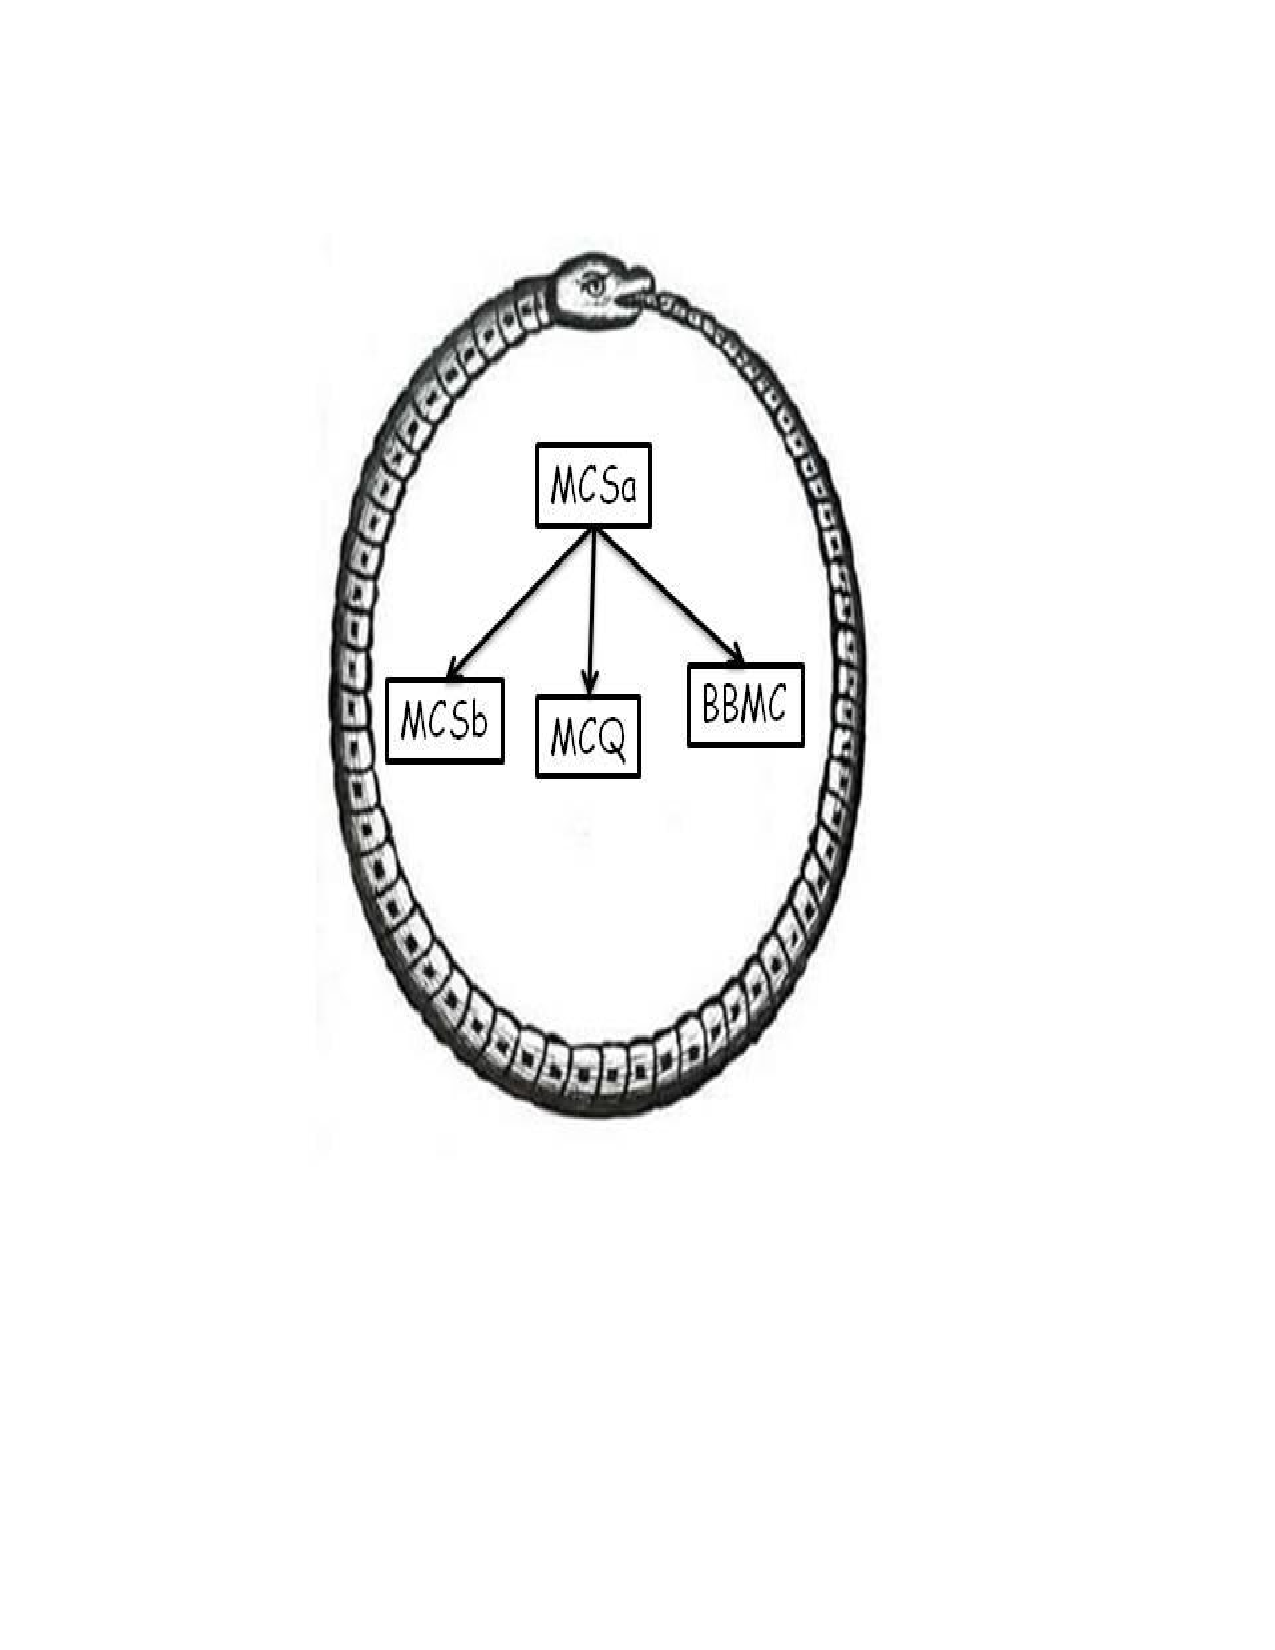
\includegraphics[height=9.2cm,width=13.2cm]{uroboros.pdf}
\vspace{-30mm}
\caption{An alternative hierarchy of the algorithms.}
\label{uroborus}
\end{figure}

The quick brown fox jumped over the \cite{ctindex} lazy dog. \cite{rdds}
The quick brown fox jumped over the lazy dog. \cite{freqStructBasedIndexing}
The quick brown fox jumped over \cite{ckt} the lazy dog.
The quick brown fox jumped over \cite{graphX} the lazy dog.

\chapter{Introduction}

    \section{Aims and motivation}
        \begin{itemize}
            \item graphs are widely used nowadays to represent data
            \item the graph containment problem is widely addressed in many areas of science: genetics, chemistry, XML documents, images, fraud detection and prevention (there was an article in nature about this)
            \item graph indexing can help us reduce the waiting time
            \item we have a lot of data that often can't be processed in memory by one machine
            \item spark is an engine that allows us to perform cluster computing and load data in-memory and share it across many clusters
            \item graphx is like spark, but has special optimizations for graphs
            \item make graph indexing in java, no concurrency and see the trade off between various indexing approaches
            \item make graph indexing in spark, vary the number of worker threads, measure performance and decide what is best
        \end{itemize}
        
        In the core of many graph-related applications, lies a common and critical problem: \textit{how to efficiently process graph queries and retrieve related graphs}. In some cases, the success of an application directly relies on the efficiency of the query processing system.  
        
        Applications:
        \begin{itemize}
        \item genome sequencing: find mutations responsible for rare diseases -- nature vol 527 no 7576
        \item treating diseases like cancer: screen a patient's tumor for a set of biomarkers to choose the best treatment to fight the particular cancer -- nature vol 527 no 7578
        \end{itemize}
\section{Background}
        
        
\section{Preliminaries}
        In this section, we introduce preliminary concepts and outline the main concepts and problems addressed in the document. In definition \ref{def:graphFormat} we explain the format of all graphs used in the document.
        
    \subsection{Naming conventions}
    \label{naming}
    - The set of target graphs: T
    - Each graph in t: $t^{}_i$, for i from 1 to the number of graphs in T
    - The set of pattern graphs: P
    - Each pattern graph in P: $p^{}_j$, for i from 1 to the number of graphs in P
    - The candidate set of graphs: C. It is important to not that C is contained in T
    - There is a trade off between the size of C and the time it takes to be computed.
        
	\subsection{Definitions}
        \begin{myDef}[Graph Format]
        \label{def:graphFormat}
        A graph G = (V, E, L, $\lambda$) is defined as an undirected labeled graph where V is the set of vertices, E is the set of edges(unordered pair of vertices), L is the set of labels, and $\lambda$ is a labeling function, $\lambda$ : V $\cup$ E $\rightarrow$ L, that assigns labels to vertices and edges.
        \end{myDef}
        
        \begin{myDef}[Graph Isomorphism]
        
        \end{myDef}

        \begin{myDef}[Subgraph Isomorphism]
        \label{def:subgraphIsomorphism}
        Given a graph database T of target graphs $t^{}_0$, $t^{}_1$, $t^{}_2$ \ldots $t^{}_i$, where \textit{i} is the number of target graphs in T, and a pattern graph P, find all targets in T that have P as a subgraph.
        \end{myDef}
        
        \begin{myDef}[Subgraph]
        \label{def:subgraph}
        A graph whose vertices and edges are a subset of another graph.
        \end{myDef}
        
        \begin{myDef}[Graph Query Processing]
        \label{def:graphQueryProcessing}
        Given a graph database D = $\{$ $g^{}_0$, $g^{}_1$, $g^{}_2$ \ldots $g^{}_n$ $\}$ and a pattern graph p, it returns the query answer set $D^{}_p$ = $\{$ $g^{}_i$$\vert$p $\subseteq$ $g^{}_i$, $g^{}_i$ $\in$ D $\}$
        
        \end{myDef}
        
        \begin{myDef}[In-memory computing]
        The storage of information in the main random access memory (RAM) of dedicated servers rather than in relational databases operating on comparatively slow disk drives.In-memory computing gives ability to cache countless amounts of data constantly. This ensures extremely fast response times for searches.
        \end{myDef}
        
        \begin{myDef} [Fault-Tolerant Manner] 
        Property that enables a system to continue to operate properly in the event of a failure.
        \end{myDef}
        
        \begin{myDef} [Cluster Computing]
        A form of computing in which a group of computers are linked together so that they can act like a single entity. 
        \end{myDef}
        
        \begin{myDef} [Graph Index]
		
		\end{myDef}
        
    \section{Graph Indexing}
        In this section, we  
        
        filter-verification process --- look at grapes
        
    \section{Data}

        
\chapter{Graph Indexing}
	\section{Motivation for usage}
	\section{Common techniques}
    	\subsection{Graph-mining}
    	\subsection{Non-graph-mining}
    \section{Methods with respect to choice of indexing unit}
        \subsection{Path-based indexing approach}
        Follows the general idea: enumerate all the existing paths in a database up to \textit{maxLen} length and index them, where a path is a vertex-edgeProperty-vetex sequence. *example*
        In order to create an index of a graph \textit{g}, this approach breaks \textit{g} into paths and in this way, the structural information of \textit{g} could be lost. This leads to more false-positive answers returned after the   
        Advantages:
        \begin{enumerate}
            \item Paths are easier to manipulate than trees and graphs.
            \item The index space is predefined: all the paths up to             \textit{maxLen} length are selected.
        \end{enumerate}
        
        Disadvantages:
        \begin{enumerate}
            \item Path is too simple: structural information is lost
            \item There are too many paths: the set of paths in a graph database usually is huge.
        \end{enumerate}
        
        
        \subsection{Tree-based indexing approach}
        
\chapter{Tools}
    \section{Spark}
        \subsection{Resilient Distributed Datasets}
    \section{GraphX}
        \subsection{The triplets}

\chapter{Implementation}
    \section{Graph input format}
    The input we are working with is a file with the following format:\newline
    
    
    
\section{CT-Index}
    
    This is an open-source implementation of the indexing algorithm from *this paper* which I haven't done myself. I use CT-Index to analyze its implementation details and use it to compare the performance of my indexing implementation and to verify the correctness of my results. CT-Index is used as a benchmark ... 
    \subsection{The idea}
    
    \subsection{Implementation}
    
    \subsection{Performance, compared to other indexing techniques}
    
    Strengths and weaknesses of this approach ...
    
    \section{IB-Index algorithms}
    All algorithms described in this section generate the candidate set of graphs in the following steps:
    
    \begin{enumerate}
        \label{indexSteps}
        \item Compute the index of all graphs in T;
        \item Compute the index of all patterns in P;
        \item Using the target and pattern indexes computed in the previous two steps, extract all graphs in T that contain all features in the pattern index;
        \item All extracted graphs from step 3 form the candidate set C.
	\end{enumerate}
    
\section{Choice of programming language}
    
    All implementations compared with CT-Index, and compared between themselves
    
\section{IB-Index 1}
    This section gives an overview of the first indexing technique that was implemented and compared with CT-Index. The following subsections describe the main idea of the algorithm, how it was implemented and its performance.
    \subsection{The idea}
        
        We enumerate exhaustively all paths for every $t$ in $T$ up to a specified maximum path length $maxLen$. The resulting paths are the index of $T$.
        
        - compute unique path for every t
        
        For example, the index of the graph on figure \ref{C5H11} consists of the paths \texttt{C, H, C-H, C-C, H-C-H, H-C-C, C-C-C} for maxLen=3.
        
        We store the extracted paths in a file. In order to compute the candidate set C of graphs in T that are to be checked for subgraph isomorphism, IB-Index does the following:

        We do the same for every \texttt{p} in \texttt{P} and store the paths in another file : \texttt{patternIndex}. After \texttt{targetIndex} and \texttt{patternIndex} are computed, we generate the candidate set \texttt{C} that contains all \texttt{t} in \texttt{T} that contain all paths, stored in \texttt{patternIndex}. \texttt{C} is the set of all graphs that might be subgraph isomorphic to the patterns in \texttt{P}. Subgraph isomorphism check needs to be computed only for the graphs in \texttt{C}. The set of target graphs  \texttt{V} isomorphic to all patterns in  \texttt{P} will be contained in  \texttt{C}.\newline

\begin{figure}[h]
\centering
\begin{minipage}{.5\textwidth}
  \centering
  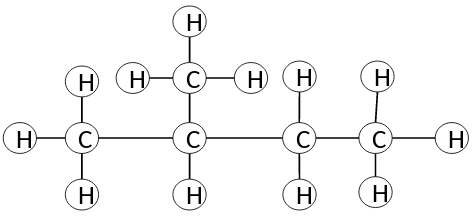
\includegraphics[height=4cm,width=9cm]{C5H11.png}
  \caption{Target Graph}
  \label{C5H11}
\end{minipage}%
\begin{minipage}{.5\textwidth}
  \centering
  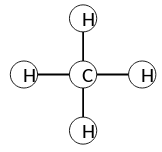
\includegraphics[height=4cm,width=4cm]{CH3.png}
  \caption{Pattern graph}
  \label{CH3}
\end{minipage}
\end{figure}

         
\subsection{Implementation}
\subsubsection{Graph representation}
	Each graph object has an integer id and is composed of a collection of node objects. Each node object has an ID, a label and a list of edge objects, where the node is a source node for each edge contained in the list. The length of the list of the edge object is equal to the degree of the node. Therefore, each edge object does not need to keep a record of the source node: it only has a label and a destination node as fields.
    
    The edge representation works for both directed and undirected graphs. If the graph is directed, only one edge object is created for each edge of the graph. If the graph is not directed, two edge objects will be created. The first one with one of the nodes as destination node and then added in the list of edges of the other node: the source node. The second edge object will have the source node of the first edge object as destination node and included in the list of edges of the destination node of the first edge object, which will be its source node. The label of both edge objects will be the same.
    
    Figure \ref{A-B} is an example of two nodes with labels A and B and an edge between them that is not labeled. To represent a directed edge, as in figure \ref{directed}, we create one Edge object with destination node B and with label an empty String. We add the created edge in node A's list of edges, as A is the source node. To represent an undirected edge, as in figure \ref{undirected}, we create two edges. Edge 1 has B as destination node and it is included in node A's list of nodes, as A is the destination node. Edge 2 has A as destination node and B as source node and consequently, it is added to the list of edges of node B, the source node.
     
\begin{figure}[h]
\centering
\begin{subfigure}{.5\textwidth}
  \centering
  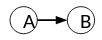
\includegraphics[height=0.8cm,width=2cm]{A-Bdirected.png}
  \caption{Directed graph}
  \label{directed}
\end{subfigure}%
\begin{subfigure}{.5\textwidth}
  \centering
  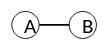
\includegraphics[height=1cm,width=2cm]{A-B.png}
  \caption{Undirected graph}
  \label{undirected}
\end{subfigure}
\caption{An edge between the nodes A and B for directed an undirected graphs}
\label{A-B}
\end{figure}
    
%%\begin{figure}[h]
%%\centering
%%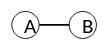
\includegraphics[height=1cm,width=2cm]{A-B.png}
%%\caption{Two nodes and an edge between them to be removed $*****$}
%%\label{A-B}
%%\end{figure}
         
\subsubsection{Path enumeration approach} %% an example

Figures \ref{C5H11-paths} and \ref{CH3-paths} show all paths of the target graph \ref{C5H11} and the pattern \ref{CH3} that will be extracted and saved in the graph index using our algorithm.

\begin{figure}[h]
\centering
\begin{subfigure}{.5\textwidth}
  \centering
  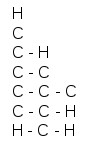
\includegraphics[height=3.5cm,width=2.5cm]{C5H11-paths.png}
  \caption{Target graph path enumeration}
  \label{C5H11-paths}
\end{subfigure}%
\begin{subfigure}{.5\textwidth}
  \centering
  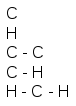
\includegraphics[height=2.5cm,width=2cm]{CH3-paths.png}
  \caption{Pattern graph path enumeration}
  \label{CH3-paths}
\end{subfigure}
\caption{All paths up to maximum length 3}
\label{A-B}
\end{figure}


Mention the bug with visited nodes and how it was fixed. Mention how the nodes that are currently on the stack are used to generate the paths.

\subsubsection{Candidates extraction}
         
            I use data structures that are not efficient -- for every node new Arraylist for edges, for every edge new object, for every graph hashmaps ...
            
            I use path-based exhaustive enumeration -- enumerate all paths up to a certain length. It is not good, because, as explained in section bla, path enumeration does not retain the graph structure
            
            The index file is very big --- compare sizes with CT-Index
\subsection{Performance}
  As this approach is very naive, we expected it to show very poor performance. The actual results were surprisingly bad. IB-Index 1 does not only run extremely slow, but it doesn't manage to filter our any of the target graphs. The index file produced contains over 8 million paths and the running time of the program is ... compared to CT-Index with running time ... !
            
\section{IB-Index 2}    
  isomers
\subsection{The idea}
        - why do I think it is better
        - picture with worked example to show that it eliminates more graphs than the first technique
       
       \subsection{Implementation}
       
       - extend IB-Index 1 and put an option to extract paths using isomer labels.
       
        \subsection{Performance}
        - the index file is bigger, but the candidate set is smaller
        
        \section{IB-Index 3}
        isomers + different graph representation (array, bitset, hashing)
        maximal paths
        


\chapter{Experimental Evaluation}
    \section{Experimental Data and Methodology}
    \section{Pure Java implementation evaluation}
    \section{Spark implementation evaluation}
    \section{Pure Java vs Spark}
    \section{Results Summary}
    
\chapter{Conclusion and Future work}

%%%%%%%%%%%%%%%%
%              %
%  APPENDICES  %
%              %
%%%%%%%%%%%%%%%%
\begin{appendices}

\chapter{Running the Programs}
An example of running from the command line is as follows:
\begin{verbatim}
      > java MaxClique BBMC1 brock200_1.clq 14400
\end{verbatim}
This will apply $BBMC$ with $style = 1$ to the first brock200 DIMACS instance allowing 14400 seconds of cpu time.

\chapter{Generating Random Graphs}
\label{sec:randomGraph}
We generate Erd\'{o}s-R\"{e}nyi random graphs $G(n,p)$ where $n$ is the number of vertices and
each edge is included in the graph with probability $p$ independent from every other edge. It produces
a random graph in DIMACS format with vertices numbered 1 to $n$ inclusive. It can be run from the command line as follows to produce 
a clq file
\begin{verbatim}
      > java RandomGraph 100 0.9 > 100-90-00.clq
\end{verbatim}
\end{appendices}

%%%%%%%%%%%%%%%%%%%%
%   BIBLIOGRAPHY   %
%%%%%%%%%%%%%%%%%%%%

\bibliographystyle{plain}
\bibliography{bib}

\end{document}
